% ===============================================================
%  جلسه شانزدهم
% ===============================================================
\chapter{یک تابع از دو متغیر تصادفی: توزیع جمع و کانولوشن}

\section{مرور: گشتاورهای مشترک، کوواریانس و همبستگی}

در جلسه قبل تعاریف زیر را دیدیم (که در این جلسه نیز به آن‌ها نیاز داریم):
\begin{itemize}
\item گشتاور مشترک مرتبه $(m,n)$: $m_{m,n}=\E(X^mY^n)$؛ با $m_{1,0}=\mu_X$، $m_{0,1}=\mu_Y$، $m_{2,0}-m_{1,0}^2=\sigma_X^2$ و $m_{0,2}-m_{0,1}^2=\sigma_Y^2$.
\item کوواریانس: $\Cov(X,Y)=\E[(X-\mu_X)(Y-\mu_Y)]=m_{1,1}-m_{1,0}m_{0,1}=\E(XY)-\mu_X\mu_Y$؛ میزان تغییرات \emph{خطی} هم‌زمان دو متغیر.
\item ضریب همبستگی (پیرسون): $\rho_{X,Y}=\frac{\Cov(X,Y)}{\sigma_X\sigma_Y}$ با $|\rho_{XY}|\le1$ (کوشی--شوارتز)، و $|\rho|=1$ اگر و تنها اگر رابطه خطی کامل.
\item $\sigma^2_{X\pm Y}=\sigma_X^2+\sigma_Y^2\pm2\rho_{XY}\sigma_X\sigma_Y$؛ برای متغیرهای مشترکاً گاوسی $\rho_{XY}=r$.
\item مستقل $\Rightarrow$ ناهمبسته؛ اما ناهمبسته $\not\Rightarrow$ مستقل (استقلال شرط بسیار قوی‌تری است).
\end{itemize}

\section{مبحث جدید: یک تابع از دو متغیر تصادفی}

\subsection{فرم کلی (تعریف مسئله)}
فرض کنید متغیرهای تصادفی $X,Y$ با توزیع مشترک $f_{XY}(x,y)$ در اختیار ما هستند. متغیر تصادفی جدید $Z=g(X,Y)$ را با استفاده از تابع یقینی $g:\R^2\to\R$ تشکیل می‌دهیم. توزیع $Z$ چگونه به دست خواهد آمد؟

\textbf{روش کلی:} مانند حالت یک متغیره، از \lr{CDF} شروع می‌کنیم:
\[
F_Z(z)=\Prob\big(g(X,Y)\le z\big)=\iint_{D_z}f_{XY}(x,y)\dd x\dd y,\qquad D_z=\{(x,y):\ g(x,y)\le z\},
\]
و سپس $f_Z=F_Z'$. یعنی باید ناحیه $D_z$ در صفحه را مشخص کرده و حجم زیر چگالی مشترک روی آن را حساب کنیم.

\section{حالت خاص: جمع $X+Y$ در حالت گسسته}

فرض کنید که دو متغیر تصادفی $X,Y$ ماهیت گسسته داشته باشند؛ یعنی داریم $X,Y\in\Z$. تابع جرم احتمال مشترک این دو را به شکل $\Prob(X=x,Y=y)$ در نظر بگیرید. همچنین، تعریف می‌کنیم $Z=g(X,Y)=X+Y$. لذا، به راحتی می‌توان دید که:
\[
\boxed{\ \Prob(Z=z)=\Prob(X+Y=z)=\sum_{t=-\infty}^{+\infty}\Prob(X=t,\ Y=z-t)\ }
\]
(رویداد $\{X+Y=z\}$ اجتماع ناسازگار رویدادهای $\{X=t,Y=z-t\}$ روی همه $t$ هاست.)

\subsection{حالت مستقل: کانولوشن گسسته}
در مسئله پیشین، همچنین فرض کنید که متغیرهای تصادفی $X,Y$ از یکدیگر \textbf{مستقل} هستند. برای سادگی در نمادگذاری، توابع $\Prob_X(\cdot),\Prob_Y(\cdot)$ را به صورت زیر تعریف می‌کنیم:
\[
\Prob_X(x)\triangleq\Prob(X=x),\qquad \Prob_Y(y)\triangleq\Prob(Y=y).
\]
در این حالت، توزیع جمع $X,Y$ برابر با \textcolor{blue!60!black}{\textbf{کانولوشن}} (\lr{Convolution}) توزیع آنان در یکدیگر خواهد شد:
\[
\boxed{\ \Prob(Z=z)=\sum_{t=-\infty}^{+\infty}\Prob_X(t)\,\Prob_Y(z-t)=\big(\Prob_X*\Prob_Y\big)(z)\ }
\]

\begin{example}[مجموع دو تاس]
\lr{PMF} مجموع دو تاس سالم و مستقل را با کانولوشن به دست آورید.
\begin{solution}
$\Prob_X(t)=\Prob_Y(t)=\frac16$ برای $t=1,\ldots,6$. برای $z\in\{2,\ldots,12\}$:
$\Prob(Z=z)=\sum_t\Prob_X(t)\Prob_Y(z-t)=\frac{1}{36}\#\{t:\ 1\le t\le6,\ 1\le z-t\le6\}=\frac{6-|z-7|}{36}$.
مثلاً $\Prob(Z=7)=\frac6{36}$ و $\Prob(Z=2)=\frac1{36}$. کانولوشن دو تابع «مستطیلی» یک تابع «مثلثی» می‌دهد.
\end{solution}
\end{example}

\begin{center}
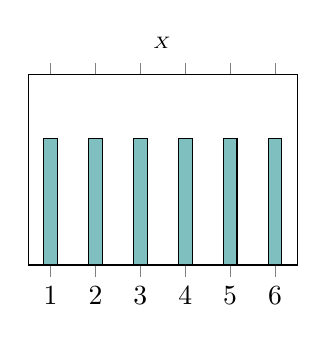
\begin{tikzpicture}
\begin{axis}[width=5cm,height=4cm,ybar,bar width=5pt,ymin=0,ymax=0.25,xtick={1,...,6},ytick=\empty,title={\small $\Prob_X$},enlarge x limits=0.1]
\addplot[fill=teal!50] coordinates {(1,0.1667) (2,0.1667) (3,0.1667) (4,0.1667) (5,0.1667) (6,0.1667)};
\end{axis}
\end{tikzpicture}
\raisebox{1.5cm}{\Large $*$}
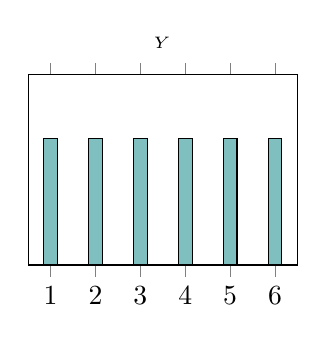
\begin{tikzpicture}
\begin{axis}[width=5cm,height=4cm,ybar,bar width=5pt,ymin=0,ymax=0.25,xtick={1,...,6},ytick=\empty,title={\small $\Prob_Y$},enlarge x limits=0.1]
\addplot[fill=teal!50] coordinates {(1,0.1667) (2,0.1667) (3,0.1667) (4,0.1667) (5,0.1667) (6,0.1667)};
\end{axis}
\end{tikzpicture}
\raisebox{1.5cm}{\Large $=$}
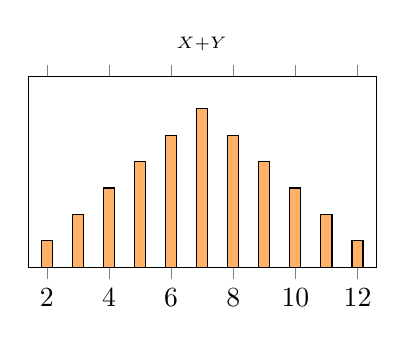
\begin{tikzpicture}
\begin{axis}[width=6cm,height=4cm,ybar,bar width=4pt,ymin=0,ymax=0.2,xtick={2,4,...,12},ytick=\empty,title={\small $\Prob_{X+Y}$},enlarge x limits=0.06]
\addplot[fill=orange!60] coordinates {(2,0.0278) (3,0.0556) (4,0.0833) (5,0.1111) (6,0.1389) (7,0.1667) (8,0.1389) (9,0.1111) (10,0.0833) (11,0.0556) (12,0.0278)};
\end{axis}
\end{tikzpicture}
\end{center}

\begin{example}[جمع دوجمله‌ای‌ها]
اگر $X\sim\mathrm{Bin}(m,p)$ و $Y\sim\mathrm{Bin}(n,p)$ مستقل باشند، $X+Y$ چه توزیعی دارد؟
\begin{solution}
با کانولوشن و اتحاد واندرموند $\sum_t\binom mt\binom n{z-t}=\binom{m+n}{z}$:
\[
\Prob(X+Y=z)=\sum_t\binom mtp^t(1-p)^{m-t}\binom n{z-t}p^{z-t}(1-p)^{n-z+t}=\binom{m+n}{z}p^z(1-p)^{m+n-z}.
\]
پس $X+Y\sim\mathrm{Bin}(m+n,p)$ ــ که شهوداً هم واضح است: $m+n$ آزمون برنولی مستقل.
\end{solution}
\end{example}

\section{حالت خاص: جمع $X+Y$ در حالت پیوسته}

حال فرض کنید، متغیرهای تصادفی $X,Y$ پیوسته باشند و با چگالی احتمال مشترک $f_{XY}(x,y)$ مدل‌سازی شوند. کماکان با فرض $Z=g(X,Y)=X+Y$، خواهیم داشت:
\[
\boxed{\ f_Z(z)=\int_\R f_{XY}(u,\ z-u)\dd u\ }
\]
و در صورتی که دو متغیر تصادفی $X,Y$ \textbf{مستقل} باشند، می‌توان دید که:
\[
\boxed{\ f_Z(z)=\int_\R f_X(u)f_Y(z-u)\dd u=\big(f_X*f_Y\big)(z)\ }
\]

\subsection{مرور توزیع جمع $X+Y$ (اثبات از طریق \lr{CDF})}
توزیع انباشته $F_{X+Y}(z)$ نیز به صورت زیر درخواهد آمد (حجم زیر چگالی مشترک روی نیم‌صفحه $x+y\le z$):
\[
F_{X+Y}(z)=\int_{-\infty}^{+\infty}\int_{-\infty}^{z-x}f_{XY}(x,y)\dd y\dd x .
\]
با مشتق‌گیری نسبت به $z$ (قاعده لایبنیتس: مشتق انتگرال درونی نسبت به حد بالای آن برابر مقدار انتگرالده در آن حد است):
\[
f_{X+Y}(z)=\int_{-\infty}^{+\infty}f_{XY}(x,z-x)\dd x ,
\]
که همان رابطه بالاست.

\begin{center}
\begin{tikzpicture}[scale=1]
\fill[cyan!40] (0,0) rectangle (2,2);
\fill[pattern=horizontal lines,pattern color=green!50!black] (0,0) -- (1.5,0) -- (0,1.5) -- cycle;
\draw[->] (-1.5,0) -- (3.5,0) node[right]{$x$};
\draw[->] (0,-1.5) -- (0,3) node[above]{$y$};
\draw[thick,brown!70!black] (-1.2,2.7) -- (2.7,-1.2) node[below right]{$x+y=z$};
\node[left,font=\small] at (0,1.5) {$z$};
\node[below,font=\small] at (1.5,0) {$z$};
\node[font=\scriptsize] at (1.2,1.4) {$f_{XY}>0$};
\end{tikzpicture}\\
{\small \lr{CDF} جمع در نقطه $z$: حجم زیر چگالی مشترک در ناحیه پایین خط $x+y=z$ (در اینجا، برای دو متغیر روی مربع واحد، ناحیه هاشورخورده).}
\end{center}

همچنین، در صورتی که متغیرهای تصادفی $X_1,X_2,\ldots$ به صورت (متقابل) مستقل از یکدیگر باشند، خواهیم داشت:
\[
f_{X_1+X_2+\cdots}(z)=\big(f_{X_1}*f_{X_2}*\cdots\big)(z).
\]

\begin{note}
\notetitle \textbf{ارتباط با \lr{MGF}:} در جلسه یازدهم دیدیم که برای متغیرهای مستقل $M_{X+Y}=M_XM_Y$. این همان «قضیه کانولوشن» است: کانولوشن در حوزه چگالی معادل ضرب در حوزه تبدیل (لاپلاس/فوریه) است. در عمل، محاسبه \lr{MGF} و ضرب آن‌ها اغلب بسیار ساده‌تر از محاسبه مستقیم انتگرال کانولوشن است.
\end{note}

\section{مثال‌ها}

\begin{example}[جمع دو یکنواخت مستقل]
فرض کنید که دو متغیر تصادفی $X,Y$ مستقل از یکدیگر بوده و هر یک توزیع یکنواخت در بازه $[0,1]$ داشته باشند. توزیع $X+Y$ را بیابید.
\begin{solution}
\[
f_Z(z)=\int_\R f_X(u)f_Y(z-u)\dd u=\int_0^1\ind_{0\le z-u\le1}\dd u .
\]
انتگرالده برابر ۱ است وقتی $u\in[0,1]$ و $u\in[z-1,z]$؛ یعنی روی اشتراک $[\max(0,z-1),\ \min(1,z)]$. طول این بازه:
\begin{itemize}
\item برای $0\le z\le1$: $[0,z]$، طول $z$؛
\item برای $1\le z\le2$: $[z-1,1]$، طول $2-z$.
\end{itemize}
\[
f_Z(z)=\begin{cases}z & 0\le z\le1\\ 2-z & 1\le z\le2\\ 0&\text{o.w.}\end{cases}
\]
یعنی جمع دو یکنواخت مستقل، توزیع \textbf{مثلثی} دارد.
\end{solution}
\end{example}

\begin{center}
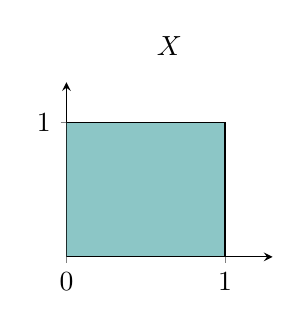
\begin{tikzpicture}
\begin{axis}[width=4.2cm,height=3.8cm,axis lines=left,xmin=0,xmax=1.3,ymin=0,ymax=1.3,xtick={0,1},ytick={1},title={$X$}]
\addplot[fill=teal!45,draw=black] coordinates {(0,0) (0,1) (1,1) (1,0)} \closedcycle;
\end{axis}
\end{tikzpicture}
\raisebox{1.3cm}{\Large $+$}
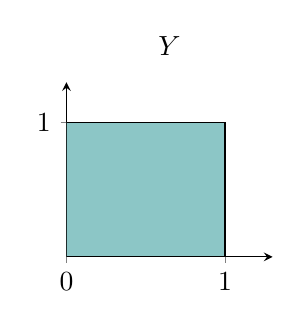
\begin{tikzpicture}
\begin{axis}[width=4.2cm,height=3.8cm,axis lines=left,xmin=0,xmax=1.3,ymin=0,ymax=1.3,xtick={0,1},ytick={1},title={$Y$}]
\addplot[fill=teal!45,draw=black] coordinates {(0,0) (0,1) (1,1) (1,0)} \closedcycle;
\end{axis}
\end{tikzpicture}
\raisebox{1.3cm}{\Large $=$}
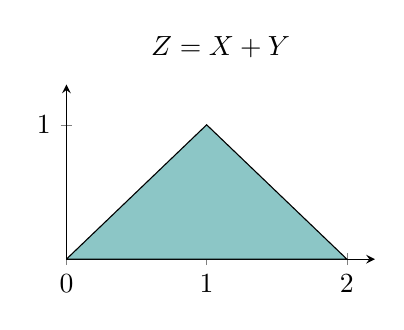
\begin{tikzpicture}
\begin{axis}[width=5.5cm,height=3.8cm,axis lines=left,xmin=0,xmax=2.2,ymin=0,ymax=1.3,xtick={0,1,2},ytick={1},title={$Z=X+Y$}]
\addplot[fill=teal!45,draw=black] coordinates {(0,0) (1,1) (2,0)} \closedcycle;
\end{axis}
\end{tikzpicture}
\end{center}

\begin{example}[جمع متغیرهای وابسته]
در سؤال قبل، فرض کنید که دو متغیر تصادفی $X,Y$ وابسته بوده و داشته باشیم $Y=2X$. حال، دوباره توزیع $X+Y$ را بیابید.
\begin{solution}
\[
Z=X+Y=3X\ \Rightarrow\ f_Z(z)=\frac13\ind_{0\le z\le3}=\mathrm{Uniform}(0,3).
\]
(از فرمول تبدیل خطی جلسه یازدهم: $f_Z(z)=\frac13f_X(\frac z3)$.) دقت کنید که اینجا حاشیه $Y$ یکنواخت روی $[0,2]$ است و \emph{نمی‌توان} از کانولوشن حاشیه‌ها استفاده کرد؛ زیرا فرمول کانولوشن فقط برای متغیرهای مستقل درست است. (با فرمول کلی $\int f_{XY}(u,z-u)\dd u$ و چگالی تکین $f_{XY}=f_X(x)\delta(y-2x)$ نیز همین جواب به دست می‌آید.)
\end{solution}
\end{example}

\begin{example}[جمع دو نمایی مستقل]
$X,Y\sim\mathrm{Exp}(\lambda)$ مستقل. توزیع $Z=X+Y$ را بیابید.
\begin{solution}
برای $z\ge0$:
\[
f_Z(z)=\int_0^z\lambda e^{-\lambda u}\lambda e^{-\lambda(z-u)}\dd u=\lambda^2e^{-\lambda z}\int_0^z\dd u=\lambda^2ze^{-\lambda z},
\]
که توزیع \textbf{ارلانگ} با $k=2$ است (جلسه هفتم). به همین ترتیب جمع $k$ نمایی مستقل، ارلانگ مرتبه $k$ است: زمان تا $k$امین رخداد در فرایند پواسون.
\end{solution}
\end{example}

\section{خواص: جمع $X+Y$ برای توزیع‌های گاوسی}

دو متغیر گاوسی $X,Y$ را با توزیع‌های حاشیه‌ای $\mathcal N(\mu,\sigma^2)$ و $\mathcal N(\mu',\sigma'^2)$ در نظر بگیرید. کماکان تعریف می‌کنیم $Z=X+Y$.

\begin{theorem}[جمع گاوسی‌های مستقل]
فرض کنید که دو متغیر تصادفی \textbf{مستقل} هستند. در این صورت می‌توان دید:
\[
f_Z=\mathcal N(\mu,\sigma^2)*\mathcal N(\mu',\sigma'^2)=\mathcal N(\mu+\mu',\ \sigma^2+\sigma'^2).
\]
\end{theorem}
\begin{proof}
با \lr{MGF}: $M_Z(t)=e^{t\mu+\sigma^2t^2/2}\,e^{t\mu'+\sigma'^2t^2/2}=e^{t(\mu+\mu')+(\sigma^2+\sigma'^2)t^2/2}$ که \lr{MGF} گاوسی با پارامترهای ادعا شده است؛ طبق یکتایی، حکم ثابت می‌شود. (اثبات مستقیم با انتگرال کانولوشن و تکمیل مربع نیز ممکن است.)
\end{proof}

\begin{note}
\notetitle توابع چگالی احتمال گاوسی، تحت عمل \lr{convolution} کماکان فرم گاوسی پیدا می‌کنند (خانواده گاوسی «بسته» به کانولوشن است). اسلاید این را این‌گونه بیان می‌کند که «توزیع گاوسی تنها توزیع با این خاصیت است»؛ به بیان دقیق‌تر: در میان توزیع‌های با \emph{واریانس متناهی}، گاوسی تنها خانواده‌ای است که جمع متغیرهای مستقل آن هم‌خانواده می‌ماند (و طبق قضیه کرامر، اگر جمع دو متغیر مستقل گاوسی باشد، هر کدام گاوسی‌اند). توزیع‌هایی مانند کوشی (با واریانس نامتناهی) نیز تحت کانولوشن بسته‌اند و به آن‌ها «توزیع‌های پایدار» می‌گویند. این خاصیت ریشه نقش ویژه گاوسی در قضیه حد مرکزی است.
\end{note}

حال فرض کنید که دو متغیر تصادفی \textbf{مشترکاً گاوسی} باشند (با ضریب همبستگی $r$). در این صورت، توزیع $Z$ کماکان یک گاوسی با میانگین $\mu+\mu'$ خواهد شد.

\begin{question}[واریانس را در این حالت (مشترکاً گاوسی) در خانه به دست آورید.]
\begin{answer}
طبق اتحاد واریانس جمع (جلسه پانزدهم) و $\rho_{XY}=r$:
\[
\Var(Z)=\sigma^2+\sigma'^2+2r\sigma\sigma'\quad\Longrightarrow\quad Z\sim\mathcal N\big(\mu+\mu',\ \sigma^2+\sigma'^2+2r\sigma\sigma'\big).
\]
برای $r=0$ به حالت مستقل می‌رسیم. حالت‌های حدی: $r=1$ و $\sigma=\sigma'$ ($Y=X$ پس از مرکزیت): واریانس $4\sigma^2=\Var(2X)$ \checkmark؛ $r=-1$ و $\sigma=\sigma'$: واریانس صفر، یعنی $Z$ ثابت است \checkmark.
\end{answer}
\end{question}

\section{تمرین‌های تکمیلی}

\begin{exercise}
$X,Y$ مستقل و هر دو یکنواخت روی $[0,1]$ هستند. توزیع $W=X-Y$ را بیابید.
\end{exercise}
\begin{solution}
$-Y$ یکنواخت روی $[-1,0]$ است و مستقل از $X$. با کانولوشن (یا با شیفت جواب مثال قبل به اندازه ۱): $f_W(w)=1-|w|$ برای $|w|\le1$ ــ مثلثی متقارن حول صفر.
\end{solution}

\begin{exercise}
$X\sim\mathrm{Pois}(2)$ و $Y\sim\mathrm{Pois}(3)$ مستقل‌اند. $\Prob(X+Y=4)$ و $\Prob(X=1\given X+Y=4)$ را بیابید.
\end{exercise}
\begin{solution}
$X+Y\sim\mathrm{Pois}(5)$، پس $\Prob(X+Y=4)=e^{-5}\frac{5^4}{24}\approx0.1755$.
$\Prob(X=1\given X+Y=4)=\frac{\Prob(X=1)\Prob(Y=3)}{\Prob(X+Y=4)}=\frac{2e^{-2}\cdot\frac{27}{6}e^{-3}}{\frac{625}{24}e^{-5}}=\frac{9\times24}{625}=0.3456$. در واقع به شرط $X+Y=n$، $X\sim\mathrm{Bin}(n,\frac{2}{5})$ و $\binom41(0.4)(0.6)^3=0.3456$ \checkmark.
\end{solution}

\begin{exercise}
$X$ و $Y$ مستقل و $\mathrm{Exp}(1)$ هستند. توزیع $Z=\max(X,Y)$ و $W=\min(X,Y)$ را بیابید.
\end{exercise}
\begin{solution}
$F_Z(z)=\Prob(X\le z,Y\le z)=(1-e^{-z})^2$ و $f_Z(z)=2e^{-z}(1-e^{-z})$ برای $z\ge0$.
$\Prob(W>w)=\Prob(X>w)\Prob(Y>w)=e^{-2w}$؛ پس $W\sim\mathrm{Exp}(2)$ (کمینه نمایی‌های مستقل، نمایی با نرخ مجموع است).
\end{solution}

\begin{exercise}
$X,Y$ مستقل و $\mathcal N(0,1)$ هستند. $\Prob(X+Y>2)$ و $\Prob(X>Y+1)$ را بیابید.
\end{exercise}
\begin{solution}
$X+Y\sim\mathcal N(0,2)$: $\Prob(X+Y>2)=1-\Phi(\frac{2}{\sqrt2})=1-\Phi(1.414)\approx0.0786$.
$X-Y\sim\mathcal N(0,2)$: $\Prob(X-Y>1)=1-\Phi(0.707)\approx0.240$.
\end{solution}
